% Options for packages loaded elsewhere
\PassOptionsToPackage{unicode}{hyperref}
\PassOptionsToPackage{hyphens}{url}
%
\documentclass[
  x11names]{article}
\usepackage{amsmath,amssymb}
\usepackage{lmodern}
\usepackage{iftex}
\ifPDFTeX
  \usepackage[T1]{fontenc}
  \usepackage[utf8]{inputenc}
  \usepackage{textcomp} % provide euro and other symbols
\else % if luatex or xetex
  \usepackage{unicode-math}
  \defaultfontfeatures{Scale=MatchLowercase}
  \defaultfontfeatures[\rmfamily]{Ligatures=TeX,Scale=1}
\fi
% Use upquote if available, for straight quotes in verbatim environments
\IfFileExists{upquote.sty}{\usepackage{upquote}}{}
\IfFileExists{microtype.sty}{% use microtype if available
  \usepackage[]{microtype}
  \UseMicrotypeSet[protrusion]{basicmath} % disable protrusion for tt fonts
}{}
\makeatletter
\@ifundefined{KOMAClassName}{% if non-KOMA class
  \IfFileExists{parskip.sty}{%
    \usepackage{parskip}
  }{% else
    \setlength{\parindent}{0pt}
    \setlength{\parskip}{6pt plus 2pt minus 1pt}}
}{% if KOMA class
  \KOMAoptions{parskip=half}}
\makeatother
\usepackage{xcolor}
\usepackage[margin=1in]{geometry}
\usepackage{graphicx}
\makeatletter
\def\maxwidth{\ifdim\Gin@nat@width>\linewidth\linewidth\else\Gin@nat@width\fi}
\def\maxheight{\ifdim\Gin@nat@height>\textheight\textheight\else\Gin@nat@height\fi}
\makeatother
% Scale images if necessary, so that they will not overflow the page
% margins by default, and it is still possible to overwrite the defaults
% using explicit options in \includegraphics[width, height, ...]{}
\setkeys{Gin}{width=\maxwidth,height=\maxheight,keepaspectratio}
% Set default figure placement to htbp
\makeatletter
\def\fps@figure{htbp}
\makeatother
\setlength{\emergencystretch}{3em} % prevent overfull lines
\providecommand{\tightlist}{%
  \setlength{\itemsep}{0pt}\setlength{\parskip}{0pt}}
\setcounter{secnumdepth}{-\maxdimen} % remove section numbering
\usepackage{fontspec} \usepackage{titling} \pretitle{\begin{center} \LARGE \vspace{-3.3cm} \includegraphics[width=\linewidth]{images/Base_info/logo.png}\\} \posttitle{\end{center}} \usepackage{framed} \usepackage{float} \usepackage{fancyhdr} \usepackage{ragged2e} \usepackage{caption} \usepackage{colortbl} \usepackage[export]{adjustbox} \usepackage{wrapfig} \captionsetup[figure]{labelformat=empty} \arrayrulecolor{white} \pagestyle{fancy} \fancyhead[L,C]{} \fancypagestyle{plain}{\pagestyle{fancy}} \PassOptionsToPackage{dvipsnames,svgnames*,x11names*}{xcolor} \definecolor{ceil}{rgb}{0.57, 0.63, 0.81}
\usepackage{booktabs}
\usepackage{longtable}
\usepackage{array}
\usepackage{multirow}
\usepackage{wrapfig}
\usepackage{float}
\usepackage{colortbl}
\usepackage{pdflscape}
\usepackage{tabu}
\usepackage{threeparttable}
\usepackage{threeparttablex}
\usepackage[normalem]{ulem}
\usepackage{makecell}
\usepackage{xcolor}
\ifLuaTeX
  \usepackage{selnolig}  % disable illegal ligatures
\fi
\IfFileExists{bookmark.sty}{\usepackage{bookmark}}{\usepackage{hyperref}}
\IfFileExists{xurl.sty}{\usepackage{xurl}}{} % add URL line breaks if available
\urlstyle{same} % disable monospaced font for URLs
\hypersetup{
  pdftitle={~},
  hidelinks,
  pdfcreator={LaTeX via pandoc}}

\title{~}
\author{}
\date{\vspace{-2.5em}}

\begin{document}
\maketitle

\renewenvironment{framed}[1][\hsize]
  {\MakeFramed{\hsize#1\advance\hsize-\width \FrameRestore}}%
  {\endMakeFramed}

\setmainfont{Arial}
\setsansfont{Arial}
\setmonofont{Arial}

\newcommand\invisiblesection[1]{%
  \refstepcounter{section}%
  \addcontentsline{toc}{section}{\protect\numberline{\thesection}#1}%
  \sectionmark{#1}}

\fancyhead[R]{\textbf{http://doi.org/10.31687/SaremLR.19.212}}

%
  \refstepcounter{section}%
  \addcontentsline{toc}{section}{\protect\numberline{\thesection}GENERALIDADES}%
  \sectionmark{GENERALIDADES}

\vspace{-3cm}

\begin{minipage}{0.7\textwidth}
\vspace{0.15cm}
{\fontsize{18}{22}\selectfont\textit{Mazama nana}}

\vspace{0.3cm}
{\fontsize{30}{36}\selectfont Corzuela enana}
\end{minipage}
\hspace{0.05\textwidth}
\begin{minipage}{0.20\textwidth}
\includegraphics[width=\textwidth]{images/nt.png}\\
\end{minipage}

\normalsize

\begin{figure}[H]

{\centering \includegraphics[width=0.9\linewidth]{photos//Cetaartiodactyla/212_Mazama-nana_1_Diego-Varela} 

}

\caption{Fotos por Roberto Cinti, Proyecto Pantano}\label{fig:image}
\end{figure}

\vspace{-1cm}

\begin{center}\rule{0.5\linewidth}{0.5pt}\end{center}

\justifying

\textbf{Citar como:} Varela, Diego. (2019). \emph{Mazama nana}. En:
SAyDS--SAREM (eds.) Categorización 2019 de los mamíferos de Argentina
según su riesgo de extinción. Lista Roja de los mamíferos de Argentina.
\url{http://doi.org/10.31687/SaremLR.19.212}

\begin{center}\rule{0.5\linewidth}{0.5pt}\end{center}

\newpage

%
  \refstepcounter{section}%
  \addcontentsline{toc}{section}{\protect\numberline{\thesection}ÁREA DE DISTRIBUCIÓN ACTUAL}%
  \sectionmark{ÁREA DE DISTRIBUCIÓN ACTUAL}
\begin{table}[H]
\centering
\begin{tabular}[t]{>{\raggedright\arraybackslash}m{16cm}>{}m{16cm}}
\toprule
\cellcolor{ceil}{\textcolor{white}{\textbf{\rule{0pt}{14pt}ÁREA DE DISTRIBUCIÓN ACTUAL}}}\\
\bottomrule
\end{tabular}
\end{table}

\vspace{-0.4cm}

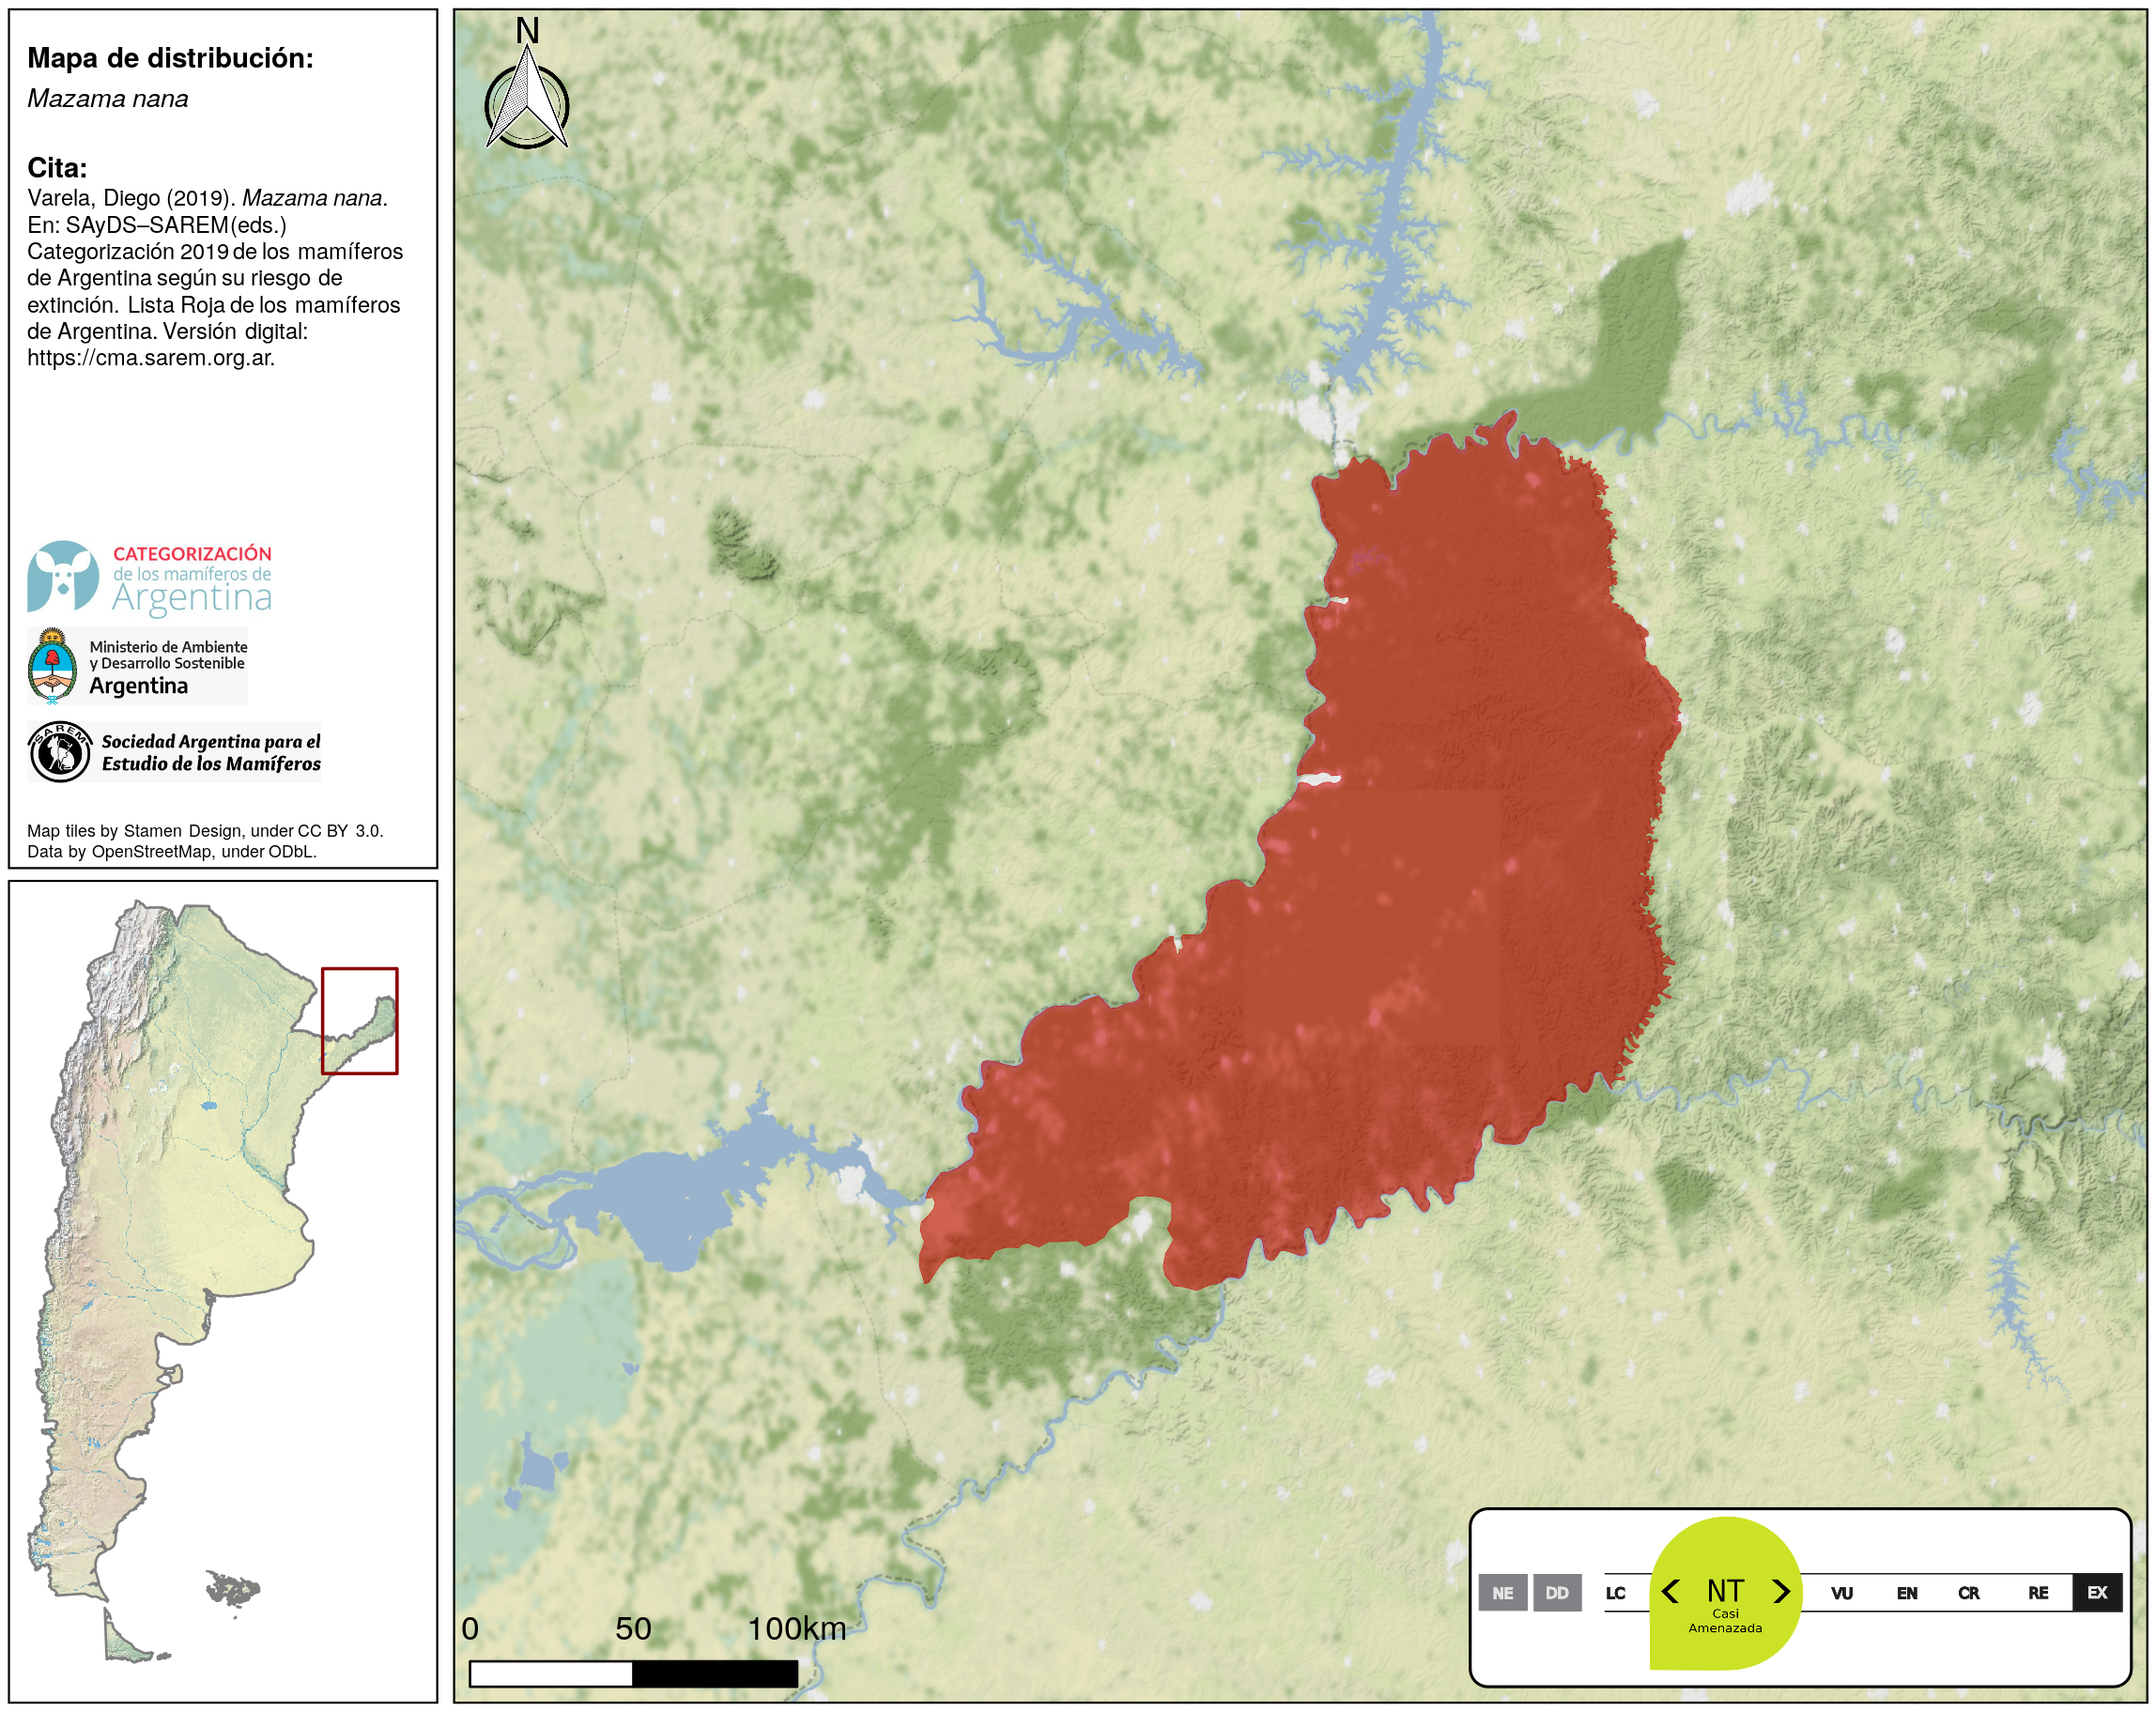
\includegraphics[width=1\linewidth]{maps/Cetartiodactyla/Mazama_nana}

%
  \refstepcounter{section}%
  \addcontentsline{toc}{section}{\protect\numberline{\thesection}CATEGORÍAS DE CONSERVACIÓN}%
  \sectionmark{CATEGORÍAS DE CONSERVACIÓN}
\begin{table}[H]
\centering
\begin{tabular}[t]{>{\raggedright\arraybackslash}m{16cm}>{}m{16cm}}
\toprule
\cellcolor{ceil}{\textcolor{white}{\textbf{\rule{0pt}{14pt}CATEGORÍAS DE CONSERVACIÓN}}}\\
\bottomrule
\end{tabular}
\end{table}

\vspace{-0.4cm}

\textbf{Categoría Nacional de Conservación 2019}

NT (Casi Amenazada)

\textbf{Criterios y subcriterios}

B1b(iii)

\textbf{Justificación de la categorización}

Mazama nana es una especie endémica de la ecorregión de la Selva
Paranaense (o Bosque Atlántico del Alto Paraná) y considerada Vulnerable
(VU) a nivel global. ~A pesar de la conversión, degradación y
fragmentación del bosque nativo en Misiones, la especie persiste en
prácticamente todo el territorio provincial. Siendo frecuente en bosques
degradados, fragmentos y en plantaciones forestales de pinos y
eucaliptus, incluso en áreas con altos niveles de caza furtiva. Es la
especie de Mazama más frecuente en monitoreos con cámaras trampa a lo
largo de la provincia de Misiones, con excepción del Parque Nacional
Iguazú donde es más frecuente Mazama americana. La especie es
categorizada como Casi Amenazada (NT) porque tiene una extensión de
presencia apenas superior a los 20.000 km2 (Criterio B1), pero no
satisface los subcriterios y condiciones. El cambio de categoría es no
genuino, y responde a una mayor información de campo sobre la especie
(monitoreos con cámaras trampa) y a una reinterpretación de los
criterios de evaluación. Sus mayores amenazas son la transformación del
bosque nativo a usos agrícolas, la caza furtiva y el hostigamiento y
depredación por perros. Se encuentra presente en la mayoría de las áreas
naturales protegidas públicas y privadas de la provincia. Es importante
destacar, que fuera del territorio argentino la especie es rara,
producto de la intensa transformación del Bosque Atlántico del Alto
Paraná para la expansión de la agricultura industrial en las regiones
vecinas de Brasil y Paraguay.

\textbf{Categoría Res. SAyDS 1030/04}

VU (Vulnerable)

\textbf{Categorías nacionales de conservación previas (SAREM)}

\begin{tabu} to \linewidth {>{}l>{\raggedright}X>{\raggedright}X}
\toprule
\textbf{\cellcolor{gray!6}{2012}} & \cellcolor{gray!6}{VU (Vulnerable)} & \cellcolor{gray!6}{B1bi,ii,iii;C1}\\
\bottomrule
\end{tabu}

\begin{tabu} to \linewidth {>{}l>{\raggedright}X>{\raggedright}X}
\toprule
\textbf{\cellcolor{gray!6}{2000}} & \cellcolor{gray!6}{VU (Vulnerable)} & \cellcolor{gray!6}{B2a+3a; C1}\\
\bottomrule
\end{tabu}

\begin{tabu} to \linewidth {>{}l>{\raggedright}X>{\raggedright}X}
\toprule
\textbf{\cellcolor{gray!6}{1997}} & \cellcolor{gray!6}{VU (Vulnerable)} & \cellcolor{gray!6}{B2a+3a; C1}\\
\bottomrule
\end{tabu}

\begin{tabu} to \linewidth {>{}l>{\raggedright}X}
\toprule
\textbf{\cellcolor{gray!6}{Homologación categoría 1997}} & \cellcolor{gray!6}{VU (Vulnerable)}\\
\bottomrule
\end{tabu}

\textbf{Categorías de conservación actuales en países vecinos}

\begin{tabu} to \linewidth {>{\raggedright}X>{\raggedright}X>{\raggedright}X>{\raggedright}X}
\toprule
\textbf{País} & \textbf{Categoría} & \textbf{Año} & \textbf{Cita}\\
\arrayrulecolor{white}
\midrule
\cellcolor{gray!6}{Brasil} & \cellcolor{gray!6}{VU (Vulnerable)} & \cellcolor{gray!6}{2018} & \cellcolor{gray!6}{ICMBio/MMA (2018)}\\
\bottomrule
\end{tabu}
\begin{tabu} to \linewidth {>{\raggedright}X>{\raggedright}X>{\raggedright}X>{\raggedright}X}
\toprule
\textbf{País} & \textbf{Categoría} & \textbf{Año} & \textbf{Cita}\\
\arrayrulecolor{white}
\midrule
\cellcolor{gray!6}{Paraguay} & \cellcolor{gray!6}{VU (Vulnerable)} & \cellcolor{gray!6}{2017} & \cellcolor{gray!6}{Saldívar et al. (2017)}\\
\bottomrule
\end{tabu}

\textbf{Evaluación global UICN}

\begin{tabu} to \linewidth {>{\raggedright}X>{\raggedright}X>{\raggedright}X}
\toprule
\textbf{Año de evaluación} & \textbf{Categoría} & \textbf{Criterios y subcriterios}\\
\arrayrulecolor{white}
\midrule
\cellcolor{gray!6}{2015} & \cellcolor{gray!6}{VU (Vulnerable)} & \cellcolor{gray!6}{A3cde}\\
\bottomrule
\end{tabu}

\arrayrulecolor{white}

%
  \refstepcounter{section}%
  \addcontentsline{toc}{section}{\protect\numberline{\thesection}TAXONOMÍA Y NOMENCLATURA}%
  \sectionmark{TAXONOMÍA Y NOMENCLATURA}
\begin{table}[H]
\centering
\begin{tabular}[t]{>{\raggedright\arraybackslash}m{16cm}>{}m{16cm}}
\toprule
\cellcolor{ceil}{\textcolor{white}{\textbf{\rule{0pt}{14pt}TAXONOMÍA Y NOMENCLATURA}}}\\
\bottomrule
\end{tabular}
\end{table}

\vspace{-0.4cm}

\begin{tabu} to \linewidth {>{\raggedright\arraybackslash}p{6cm}>{\raggedright\arraybackslash}p{1cm}>{\raggedright}X}
\toprule
\textbf{\cellcolor{gray!6}{Orden}} & \cellcolor{gray!6}{} & \cellcolor{gray!6}{Cetartiodactyla}\\
\bottomrule
\end{tabu} \vspace{0.3cm}
\begin{tabu} to \linewidth {>{\raggedright\arraybackslash}p{6cm}>{\raggedright\arraybackslash}p{1cm}>{\raggedright}X}
\toprule
\textbf{\cellcolor{gray!6}{Familia}} & \cellcolor{gray!6}{} & \cellcolor{gray!6}{Cervidae}\\
\bottomrule
\end{tabu} \vspace{0.3cm}
\begin{tabu} to \linewidth {>{\raggedright\arraybackslash}p{6cm}>{\raggedright\arraybackslash}p{1cm}>{\raggedright}X}
\toprule
\textbf{\cellcolor{gray!6}{Nombre científico}} & \cellcolor{gray!6}{} & \cellcolor{gray!6}{\textit{Mazama nana} (Hensel, 1872)}\\
\bottomrule
\end{tabu} \vspace{0.3cm}
\begin{tabu} to \linewidth {>{\raggedright\arraybackslash}p{6cm}>{\raggedright\arraybackslash}p{1cm}>{\raggedright}X}
\toprule
\textbf{\cellcolor{gray!6}{Nombre común}} & \cellcolor{gray!6}{} & \cellcolor{gray!6}{Corzuela enana}\\
\bottomrule
\end{tabu} \vspace{0.3cm}
\begin{tabu} to \linewidth {>{\raggedright\arraybackslash}p{6cm}>{\raggedright\arraybackslash}p{1cm}>{\raggedright}X}
\toprule
\textbf{\cellcolor{gray!6}{Nombres comunes locales}} & \cellcolor{gray!6}{} & \cellcolor{gray!6}{Poca}\\
\textbf{} &  & Poquita\\
\textbf{\cellcolor{gray!6}{}} & \cellcolor{gray!6}{} & \cellcolor{gray!6}{Pororó}\\
\textbf{} &  & Mbororó\\
\textbf{\cellcolor{gray!6}{}} & \cellcolor{gray!6}{} & \cellcolor{gray!6}{Pororoka}\\
\bottomrule
\end{tabu} \vspace{0.3cm}
\begin{tabu} to \linewidth {>{\raggedright\arraybackslash}p{6cm}>{\raggedright\arraybackslash}p{1cm}>{\raggedright}X}
\toprule
\textbf{\cellcolor{gray!6}{Nombres comunes en inglés}} & \cellcolor{gray!6}{} & \cellcolor{gray!6}{Brazilian Dwarf Brocket}\\
\textbf{} &  & Pygmy Brocket\\
\bottomrule
\end{tabu} \vspace{0.3cm}
\begin{tabu} to \linewidth {>{\raggedright\arraybackslash}p{6cm}>{\raggedright\arraybackslash}p{1cm}>{\raggedright}X}
\toprule
\textbf{\cellcolor{gray!6}{Nombres comunes en portugués}} & \cellcolor{gray!6}{} & \cellcolor{gray!6}{Veado-cambuta}\\
\textbf{} &  & Veado-mao-curta\\
\textbf{\cellcolor{gray!6}{}} & \cellcolor{gray!6}{} & \cellcolor{gray!6}{Veado-poca}\\
\textbf{} &  & Veado bororó do sul\\
\bottomrule
\end{tabu} \vspace{0.3cm}

\textbf{Comentarios taxonómicos}

Sinónimos: \textit{Mazama} \textit{nana} (Czernay, 1987) Mazama rufina
nana (Cabrera, 1960) Mazama rufina (Vieira, 1955)

\arrayrulecolor{white}

%
  \refstepcounter{section}%
  \addcontentsline{toc}{section}{\protect\numberline{\thesection}INFORMACIÓN RELEVANTE PARA LA EVALUACIÓN}%
  \sectionmark{INFORMACIÓN RELEVANTE PARA LA EVALUACIÓN}
\begin{table}[H]
\centering
\begin{tabular}[t]{>{\raggedright\arraybackslash}m{16cm}>{}m{16cm}}
\toprule
\cellcolor{ceil}{\textcolor{white}{\textbf{\rule{0pt}{14pt}INFORMACIÓN RELEVANTE PARA LA EVALUACIÓN}}}\\
\bottomrule
\end{tabular}
\end{table}

\vspace{-0.4cm}

%
  \refstepcounter{section}%
  \addcontentsline{toc}{section}{\protect\numberline{\thesection}RANGO GEOGRÁFICO, OCURRENCIA Y ABUNDANCIA}%
  \sectionmark{RANGO GEOGRÁFICO, OCURRENCIA Y ABUNDANCIA}
\begin{table}[H]
\centering
\begin{tabular}[t]{>{\raggedright\arraybackslash}m{16cm}>{}m{16cm}}
\toprule
\cellcolor{ceil}{\textcolor{white}{\textbf{\rule{0pt}{14pt}RANGO GEOGRÁFICO, OCURRENCIA Y ABUNDANCIA}}}\\
\bottomrule
\end{tabular}
\end{table}

\vspace{-0.4cm}

\textbf{Presencia en el territorio nacional:} residente

\textbf{Comentarios sobre la distribución actual e histórica}

La especie es endémica de la ecorregión del Bosque Atlántico del Alto
Paraná de Brasil, Paraguay y Argentina (Abril et al.~2010; de Oliveira
et al.~2019). En la provincia de Misiones ha sido registrada en áreas de
bosque nativo con vegetación densa, abundante cubierta de bambú y
bosques secundarios, conocidos como ``capueras'' (Chébez \& Varela 2001;
Massoia et al.~2006). Asimismo, se ha~registrado que utiliza
las~plantaciones forestales que se extienden a lo largo de la provincia.
El límite de distribución mas austral es incierto para Argentina, pero
en la porción sur de la provincia de Misiones la especie es
frecuentemente desplazada por su congénere Mazama gouazoubira.~

\begin{tabu} to \linewidth {>{\raggedright\arraybackslash}p{8cm}>{\raggedright\arraybackslash}p{0.5cm}>{\raggedright}X}
\toprule
\textbf{\cellcolor{gray!6}{Presencia confirmada por provincia:}} & \cellcolor{gray!6}{} & \cellcolor{gray!6}{Misiones}\\
\bottomrule
\end{tabu}

\begin{tabu} to \linewidth {>{\raggedright\arraybackslash}p{8cm}>{\raggedright\arraybackslash}p{0.5cm}>{\raggedright}X}
\toprule
\textbf{\cellcolor{gray!6}{Presencia en ecorregiones de Argentina:}} & \cellcolor{gray!6}{} & \cellcolor{gray!6}{Selva Paranaense}\\
\bottomrule
\end{tabu}

\begin{tabu} to \linewidth {>{\raggedright\arraybackslash}p{8cm}>{\raggedright\arraybackslash}p{0.5cm}>{\raggedright}X}
\toprule
\textbf{\cellcolor{gray!6}{Presencia en ecorregiones globales terrestres:}} & \cellcolor{gray!6}{} & \cellcolor{gray!6}{ID439 – Bosque Atlántico del Alto Paraná}\\
\textbf{} &  & ID440 – Bosques Húmedos de Araucaria\\
\bottomrule
\end{tabu}

\begin{tabu} to \linewidth {>{\raggedright}X>{\raggedright}X>{\raggedright}X}
\toprule
\textbf{Patrón de distribución} & \textbf{Cantidad de localidades} & \textbf{Rango altitudinal}\\
\midrule
\cellcolor{gray!6}{continuo} & \cellcolor{gray!6}{NA} & \cellcolor{gray!6}{100-500 msnm}\\
\bottomrule
\end{tabu}

\begin{tabu} to \linewidth {>{}l>{\raggedright}X}
\toprule
\textbf{\cellcolor{gray!6}{Endemismo}} & \cellcolor{gray!6}{especie endémica ecorregional}\\
\bottomrule
\end{tabu}

\begin{tabu} to \linewidth {>{}l>{\raggedright}X}
\toprule
\textbf{\cellcolor{gray!6}{Abundancia relativa estimada en su área de ocupación}} & \cellcolor{gray!6}{frecuente}\\
\bottomrule
\end{tabu}

\textbf{Comentarios sobre la abundancia, densidad o probabilidad de
ocupación de la especie}

La especie es relativamente frecuente en todos los remanentes de bosque
nativo del centro y norte de Misiones, incluso en plantaciones
forestales de pinos y eucalyptus. En áreas fragmentadas, quebradas y
menos protegidas, M. nana es mas abundante que M. americana (Di Bitetti
et al.~2008;~Paviolo et al.~2009, 2018).

\textbf{¿Existen actualmente programas de monitoreo?:} sí

El centro y norte de Misiones es monitoreado por el IBS (CONICET-UNaM) a
traves de varios proyectos con cámaras trampa.

\arrayrulecolor{white}

%
  \refstepcounter{section}%
  \addcontentsline{toc}{section}{\protect\numberline{\thesection}DATOS MORFOMÉTRICOS}%
  \sectionmark{DATOS MORFOMÉTRICOS}
\begin{table}[H]
\centering
\begin{tabular}[t]{>{\raggedright\arraybackslash}m{16cm}>{}m{16cm}}
\toprule
\cellcolor{ceil}{\textcolor{white}{\textbf{\rule{0pt}{14pt}DATOS MORFOMÉTRICOS}}}\\
\bottomrule
\end{tabular}
\end{table}

\vspace{-0.4cm}

\begin{tabu} to \linewidth {>{\raggedright}X}
\toprule
\textbf{Peso}\\
\midrule
\cellcolor{gray!6}{8-12 kg}\\
\bottomrule
\end{tabu}

\arrayrulecolor{white}

%
  \refstepcounter{section}%
  \addcontentsline{toc}{section}{\protect\numberline{\thesection}RASGOS ETO-ECOLÓGICOS}%
  \sectionmark{RASGOS ETO-ECOLÓGICOS}
\begin{table}[H]
\centering
\begin{tabular}[t]{>{\raggedright\arraybackslash}m{16cm}>{}m{16cm}}
\toprule
\cellcolor{ceil}{\textcolor{white}{\textbf{\rule{0pt}{14pt}RASGOS ETO-ECOLÓGICOS}}}\\
\bottomrule
\end{tabular}
\end{table}

\vspace{-0.4cm}

\textbf{Hábitos:} terrestres

\textbf{Hábitos especializados:} cursorial

\textbf{Otro hábito especializado: comentarios}

NA

\textbf{Dieta:} herbívoro

\textbf{Dieta especializada:} frugívoro, folívoro

\textbf{Aspectos reproductivos}

Se desconocen prácticamente los aspectos reproductivos para las
poblaciones de Argentina. Algunas referencias, mencionan un período de
gestación de tres meses, con nacimientos de una sola cría,
principalmente entre los meses de septiembre y febrero (Crespo 1982,
Massoia et al.~2006). Sin embargo, otros autores mencionan~que el
período de gestación es de aproximadamente siete meses y presencia de
estro posparto (Abril et al.~2010).

\textbf{Patrón de actividad:} catemeral

\textbf{Gregariedad:} especie solitaria

NA

\textbf{Área de acción}

Si bien no existe información específica~sobre la ecología de la
especie,~probablemente sus áreas de acción sean pequeñas (Abril et
al.~2010).

%
  \refstepcounter{section}%
  \addcontentsline{toc}{section}{\protect\numberline{\thesection}CONSERVACIÓN E INVESTIGACIÓN}%
  \sectionmark{CONSERVACIÓN E INVESTIGACIÓN}
\begin{table}[H]
\centering
\begin{tabular}[t]{>{\raggedright\arraybackslash}m{16cm}>{}m{16cm}}
\toprule
\cellcolor{ceil}{\textcolor{white}{\textbf{\rule{0pt}{14pt}CONSERVACIÓN E INVESTIGACIÓN}}}\\
\bottomrule
\end{tabular}
\end{table}

\vspace{-0.4cm}

\textbf{Amenazas por grado: de 1 (menor) a 5 (mayor)}

\begin{tabu} to \linewidth {>{}l>{\raggedright}X>{}l>{\raggedright}X}
\toprule
\textbf{\cellcolor{gray!6}{Fragmentación de poblaciones}} & \cellcolor{gray!6}{1} & \textbf{\cellcolor{gray!6}{Pérdida de hábitat}} & \cellcolor{gray!6}{5}\\
\textbf{Atropellamiento en rutas} & 3 & \textbf{Depredación por perros} & 5\\
\textbf{\cellcolor{gray!6}{Enfermedades}} & \cellcolor{gray!6}{3} & \textbf{\cellcolor{gray!6}{}} & \cellcolor{gray!6}{}\\
\bottomrule
\end{tabu}

La corzuela e\textit{nana} es una especie cazada ilegalmente por los
pobladores locales para consumo de carne. Es muy vulnerable a la
depredación por perros, con muchos registros de hostigamiento y muerte
de animales en fragmentos de bosque de Misiones. Se han registrado
atropellamientos en las rutas de la provincia, tanto~dentro como fuera
de áreas protegidas (Bauni et al.~2017).

En Brasil, el virus de la lengua azul está involucrado en brotes de
enfermedades hemorrágicas en diferentes especies de cérvidos (Kawanami
et al.~2018), y recientemente se ha demostrado que las poblaciones de~M.
nana pueden verse afectadas por~este virus (Baldini et al.~2018).

\textbf{La especie ¿está presente en áreas naturales protegidas?:} sí

\textbf{Presencia de la especie en áreas naturales protegidas}

Misiones: PN Iguazú, Reserva Natural Estricta San Antonio, PP Península,
Reserva Privada de Usos Múltiples Valle del Cuña Pirú (UNLP), PP Salto
Encantado y Valle de Cuñá Pirú, PP Horacio Foerster, PP Segismundo
Welcz, PP Moconá, PP Esmeralda, Reserva de Usos Múltiples Guaraní, PP
Yacuy.PP Piñalito, Reserva de Biosfera Yabotí.

Numerosas reservas naturales privadas de Misiones, como RVS Urugua-í,
Rubichana, En las reservas privadas del Corredor Biológico Urugua-i -
Foerster: Yate-í, Karadya, San Sebastian de la Selva, San José, San
Francisco, Yvytú, Los Tatetos, Reserva Natural Urutaú.

\textbf{Marco legal de la especie}

\textbf{Planes de acción y/o proyectos de conservación o manejo
actuales}

\textbf{Experiencias de reintroducción o erradicación:} no

\textbf{Rol ecológico / servicios ecosistémicos}

Como en otras especies del género \textit{Mazama}, la especie es
potencial dispersora de semillas.

\textbf{Necesidades de investigación y conocimiento}

Es uno de los cérvidos menos estudiados de América. Se conoce muy poco
de su biología y ecología.

\arrayrulecolor{white}

%
  \refstepcounter{section}%
  \addcontentsline{toc}{section}{\protect\numberline{\thesection}BIBLIOGRAFÍA}%
  \sectionmark{BIBLIOGRAFÍA}
\begin{table}[H]
\centering
\begin{tabular}[t]{>{\raggedright\arraybackslash}m{16cm}>{}m{16cm}}
\toprule
\cellcolor{ceil}{\textcolor{white}{\textbf{\rule{0pt}{14pt}BIBLIOGRAFÍA}}}\\
\bottomrule
\end{tabular}
\end{table}

\vspace{-0.4cm}

\setlength{\parindent}{20pt}\noindent\textbf{LITERATURA CITADA}

ABRIL, V. V., A. VOGLIOTTI, D. M. VARELA, J. M. B. DUARTE, \& J. L.
CARTES. 2010. Brazilian Dwarf Brocket Deer \textit{Mazama} \textit{nana}
(Hensel 1872). Neotropical cervidology: biology and medicine of
Neotropical deer (J. M. B. Duarte \& S. González, eds.). FUNEP and IUCN,
Jaboticabal.

BALDINI, M. H. M. ET AL. 2018. Multiple bluetongue virus serotypes
causing death in Brazilian dwarf brocket deer (\textit{Mazama}
\textit{nana}) in Brazil, 2015--2016. Veterinary Microbiology
227:143--147.

BAUNI, V., J. ANFUSO, \& F. SCHIVO. 2017. Mortalidad de fauna silvestre
por atropellamientos en el bosque atlántico del Alto Paraná, Argentina.
Revista Ecosistemas 26:54--66.

DI BITETTI, M. S., A. PAVIOLO, C. FERRARI, C. DE ANGELO, \& Y. DI
BLANCO. 2008. Differential responses to hunting in two sympatric species
of brocket deer (\textit{Mazama} americana and M. \textit{nana}).
Biotropica 40:636--645.

CHÉBEZ, J. C., \& D. M. VARELA. 2001 Corzuela e\textit{nana}. Los
ciervos autóctonos de la Argentina (C. M. Dellafiore \& N. Macieira,
eds.). Buenos Aires, GAC.

CIRIGNOLI, S., C. A. GALLIARI, U. F. PARDIÑAS, D. H. PODESTÁ, \& R.
ABRAMSON. 2011. Mamíferos de la Reserva Valle del Cuña Pirú, Misiones,
Argentina. Mastozoología Neotropical 18:25--43.

CRESPO, J. A. 1982. Ecología de la comunidad de mamíferos del Parque
Nacional Iguazú, Misiones. Revista del Museo Argentino de Ciencias
Naturales ``Bernardino Rivadavia'', Ecología 3:45--162.

DE OLIVEIRA, M. L., H. T. Z. DO COUTO, \& J. M. B. DUARTE. 2019.
Distribution of the elusive and threatened Brazilian dwarf brocket deer
refined by non-invasive genetic sampling and distribution modelling.
European Journal of Wildlife Research 65:21.

DUARTE, J. M. B., A. VOGLIOTTI, J. L. CARTES, \& M. L. OLIVEIRA. 2015.
\textit{Mazama} \textit{nana}. The IUCN Red List of Threatened Species
2015: e.T29621A22154379.

ICMBio/MMA. 2018. Livro Vermelho da Fauna Brasileira Ameaçada de
Extinção: Volume I. 1ra. ed.~Brasília, DF.

KAWANAMI, A. E., J. P. DE OLIVEIRA, A. ARENALES, B. CROSSLEY, L. W.
WOODS, J. M. B. DUARTE, \& K. WERTHER. 2018. Detection of bluetongue
virus in Brazilian cervids in São Paulo state. Pesquisa Veterinária
Brasileira 38:137--142.

MASSOIA, E., J. C. CHEBEZ, \& A. BOSSO. 2006. Los mamíferos silvestres
de la provincia de Misiones, Argentina. Edición de los autores, Buenos
Aires.

PACIFICI, M. ET AL. 2013. Generation length for mammals. Nature
Conservation 5:8--94.

PAVIOLO, A. ET AL. 2009. Efecto de la caza y el nivel de protección en
la abundancia de los grandes mamíferos del Bosque Atlántico de
Misiones.~Contribuciones para la Conservación y Manejo en el Parque
Nacional Iguazú (B. Carpinetti, \& M. Garciarena, eds.). Administración
de Parques Nacionales, Buenos Aires, Argentina.

PAVIOLO, A. ET AL. 2018. Barriers, corridors or suitable habitat? Effect
of monoculture tree plantations on the habitat use and prey availability
for jaguars and pumas in the Atlantic Forest. Forest Ecology and
Management 430:576--586.

SALDÍVAR, S. ET AL. 2017. Los Mamíferos Amenazados del Paraguay. Libro
Rojo de los Mamíferos del Paraguay: especies amenazadas de extinción (S.
Saldívar, V. Rojas \& D. Giménez, eds.). Asociación Paraguaya de
Mastozoología y Secretaría del Ambiente. CREATIO, Asunsión.

\noindent\textbf{LITERATURA DE REFERENCIA}

ABRIL, V. V., \& J. M. B. DUARTE. 2008. Chromosome polymorphism in the
Brazilian dwarf red brocket deer, \textit{Mazama} \textit{nana}
(Mammalia, Cervidae). Genetics and Molecular Biology 31:53--57.

CANEVARI, M., \& O. VACCARO. 2007. Guía de mamíferos del sur de América
del Sur.~ L.O.L.A, Buenos Aires.

DUARTE, J. M. B. ET AL. 2012. Avaliação do risco de extinção do
veado-cambuta \textit{Mazama} \textit{nana} Hensel, 1872, no Brasil.
Biodiversidade Brasileira 2:59--67.

FERRARI, C. 2006. Abundancia, uso del hábitat y patrones de actividad
del venado pardo (\textit{Mazama} americana) y la poca (Mazama
\textit{nana}) en la Selva Paranaense. Tesis de Licenciatura.
Universidad Nacional de Mar del Plata, Buenos Aires.

MATTIOLI, S. 2011. Familia Cervidae. Handbook of the Mammals of the
World - Volume 2. Hoofed Mammals (D. E. Wilson \& R. A. Mittermeier,
eds.). Lynx Edicions, Barcelona.

\setlength{\parindent}{0pt}

%
  \refstepcounter{section}%
  \addcontentsline{toc}{section}{\protect\numberline{\thesection}AUTORES}%
  \sectionmark{AUTORES}
\begin{table}[H]
\centering
\begin{tabular}[t]{>{\raggedright\arraybackslash}m{16cm}>{}m{16cm}}
\toprule
\cellcolor{ceil}{\textcolor{white}{\textbf{\rule{0pt}{14pt}AUTORES}}}\\
\bottomrule
\end{tabular}
\end{table}

\vspace{-0.4cm}

\textbf{AUTORES}

\begin{longtabu} to \linewidth {>{\raggedright\arraybackslash}p{5cm}>{\raggedright\arraybackslash}p{1cm}>{\raggedright\arraybackslash}p{9cm}}
\toprule
\textbf{\cellcolor{gray!6}{\begin{justify}Varela, Diego\end{justify}}} & \cellcolor{gray!6}{} & \cellcolor{gray!6}{\begin{justify} Instituto de Biología Subtropical (IBS), CONICET-Universidad Nacional de Misiones y Centro de Investigaciones del Bosque Atlántico (CeIBA), Puerto Iguazú, Misiones, Argentina \end{justify}}\\
\bottomrule
\end{longtabu}

\textbf{COLABORADORES}

\begin{longtabu} to \linewidth {>{\raggedright\arraybackslash}p{5cm}>{\raggedright\arraybackslash}p{1cm}>{\raggedright\arraybackslash}p{9cm}}
\toprule
\textbf{\cellcolor{gray!6}{\begin{justify}Cirignoli, Sebastián\end{justify}}} & \cellcolor{gray!6}{} & \cellcolor{gray!6}{\begin{justify}Centro de Investigaciones del Bosque Atlántico (CeIBA), Puerto Iguazú, Misiones, Argentina\end{justify}}\\
\textbf{\begin{justify}Torresín, Jerónimo\end{justify}} &  & \begin{justify}Fundación Temaikén, Posadas, Misiones, Argentina\end{justify}\\
\bottomrule
\end{longtabu}

\begin{Center}
\bgroup \MakeFramed{\hsize 0.7\textwidth\advance\hsize-\width \FrameRestore}
  \begin{minipage}{\linewidth}
    \Centering
    \small
  Este documento fue generado automáticamente\\
  Fecha de compilación: 2023-04-07 19:36:03\\
  La reproducción sin cambios de este documento está permitida\\
  Si encuentra errores por favor escribir a comisioncma@sarem.com\\
  \end{minipage}
\endMakeFramed\egroup 
\end{Center}

\end{document}
